\section{Poisson solver}
\label{sec:poisson}
\renewcommand{\thesubsection}{\thesection.\arabic{subsection}}
In this section of the lab report, we will dicuss a prallel implementation of the Poisson solver. The Poisson solver is a numerical method used to solve the Poisson equation, which is a partial differential equation that is useful in many areas of physics. \\
\textbf{Note:} For local testing and development I'll run the code with \texttt{mpirun} instead of the \texttt{srun} command on the cluster. \\

\subsection{Building a parallel Poisson solver}
For the first part of the exercise we follow the steps lined out in the assignment sheet. I'll comment on the steps 1 through 10 and related questions bellow. The finished implementation can be found in the appendix for this section. \\
\begin{enumerate}
    \item \textbf{Step:} After adding MPI\_Init and MPI\_Finalize, we can run the program with multiple processes. We can see that the program runs with 4 processes in \autoref{fig:poisson_step1} via the quadrupeled output.
    \begin{figure}[H]
        \centering
        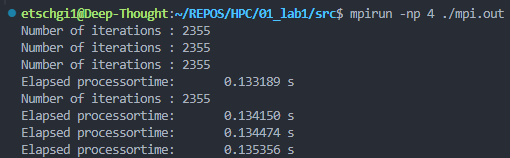
\includegraphics[width=0.5\textwidth]{../fig/lab1/step1.png}
        \caption{MPI\_Poisson after Step 1 - Running with 4 processes}
        \label{fig:poisson_step1}
    \end{figure}
    \item \textbf{Step:} To see which process is doing what, I included the rank of the process for the print statements as shown in \autoref{fig:poisson_step2}.
    \begin{figure}[H]
        \centering
        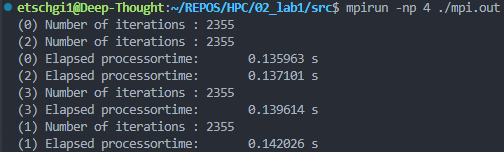
\includegraphics[width=0.5\textwidth]{../fig/lab1/step2.png}
        \caption{MPI\_Poisson after Step 2 - Running with 4 processes}
        \label{fig:poisson_step2}
    \end{figure}
    \item \textbf{Step:} Next we define \texttt{wtime} as a global double and replace the four utility timing functions with the ones given on Brightspace. A quick verification as shown in \autoref{fig:poisson_step3} shows that the program still runs as expected.
    \begin{figure}[H]
        \centering
        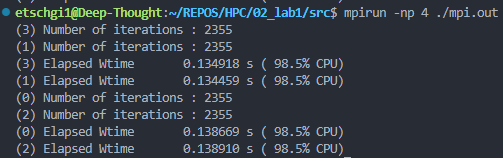
\includegraphics[width=0.5\textwidth]{../fig/lab1/step3.png}
        \caption{MPI\_Poisson after Step 3 - Running with 4 processes}
        \label{fig:poisson_step3}
    \end{figure}
    \item \textbf{Step:} Next we check if two processes indeed give the same output. Both need 2355 iterations to converge and the \texttt{diff} command returned no output, which means that the files content is identical. 
    \item \textbf{Step:} Now only the process with rank 0 will read data from files and subsequently broadcast it to the others. Testing this again with 2 processes, we see an empty diff of the output files and the same number of iterations needed to converge.
    \item \textbf{Step:} We create a cartesian grid of processes using \texttt{MPI\_Cart\_create} and use \texttt{MPI\_Cart\_shift} to find the neighbors of each process. We can see that the neighbors are correctly identified in \autoref{fig:poisson_step6}. 
    \begin{figure}[H]
        \centering
        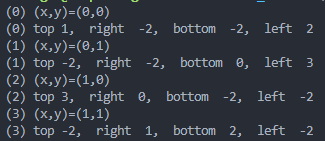
\includegraphics[width=0.5\textwidth]{../fig/lab1/step6.png}
        \caption{MPI\_Poisson after Step 6 - Running with 4 processes on a 2x2 grid}
        \label{fig:poisson_step6}
    \end{figure}
    When there is no neighbor in a certain direction, -2 (or \texttt{MPI\_PROC\_NULL}) is returned. 
    \item \textbf{Step:} We overhaul the setup to get a proper local grid for each process. Furthermore, we only save the relevant source fields in the local grid for each process. \\
    \Shining{With for instance 3 processes you should see that 1 or 2 processes do not do any 
    iteration. Do you understand why?}\\
    If we have a look at the input file we see that there are only 3 source fields in the grid. This means that the process that does not have a source field in its local grid will not do any iterations (or only 1). Therefore, if we have 3 processes and the distribution of source fields as given in the input file only 1 process will do iterations if processes are ordered in x-direction and 2 if ordered in y-direction. From this we can conclude that indeed all processes have different local grids and perform different calculations. 
    \begin{figure}[H]
        \centering
        \begin{minipage}{0.48\textwidth}
            \centering
            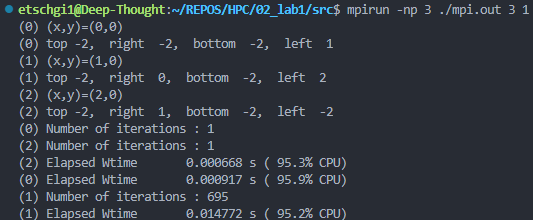
\includegraphics[width=\linewidth]{../fig/lab1/step7a.png}
        \end{minipage}%
        \hspace{0.02\textwidth}
        \begin{minipage}{0.48\textwidth}
            \centering
            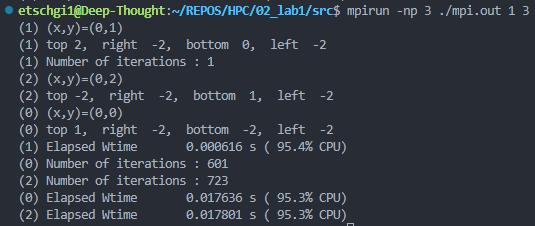
\includegraphics[width=\linewidth]{../fig/lab1/step7b.png}
        \end{minipage}
        \caption{MPI\_Poisson after Step 7 - Running with 3 processes on a 3x1 (left) vs. 1x3 (right) grid\\For the 3x1 grid, only rank 1 does iterations ($> 1$), for the 1x3 grid, ranks 0 and 2 do iterations ($> 1$).}
        \label{fig:poisson_step7}
    \end{figure}
    \item \textbf{Step:} After defining and commiting two special datatypes for vertical and horizontal communication, we setup the communication logic to exchange the boundary values between the processes. We call our \texttt{Exchange\_Borders} function after each iteration (for both red / black grid points). Now we face the problem in which some processes may stop instantly (no source in their local grid). They will not supply any data to their neighbors, which will cause the program to hang. We shall fix this in the next step.
    \item \textbf{Step:} Finally we need to implement the logic to check for convergence (in a global sense). We do this by using a \texttt{MPI\_Allreduce} call with the \texttt{MPI\_SUM} operation. This way we aggregate all deltas into one global delta which we use in the while-loop-condition to check for convergence. We can see that the program now runs as expected in \autoref{fig:poisson_step9}.
    \begin{figure}[H]
        \centering
        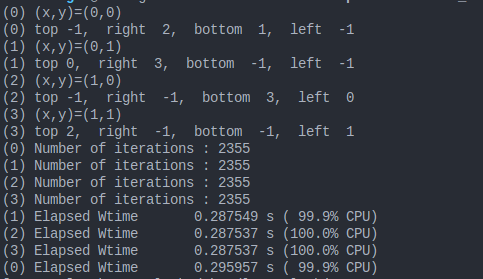
\includegraphics[width=0.5\textwidth]{../fig/lab1/step9.png}
        \caption{MPI\_Poisson after Step 9 - Running with 4 processes on a 2x2 grid}
        \label{fig:poisson_step9}
    \end{figure}
    \TODO{Different iteration count between seq and parallel version?! - also change pic if fixed.}
    \item \textbf{Step:} 
\end{enumerate}
